\documentclass[12pt]{report}
\usepackage[utf8]{inputenc}
\usepackage[russian]{babel}
%\usepackage[14pt]{extsizes}
\usepackage{listings}
\usepackage{graphicx}
\usepackage{amsmath,amsfonts,amssymb,amsthm,mathtools} 
\usepackage{pgfplots}
\usepackage{filecontents}
\usepackage{indentfirst}
\usepackage{eucal}
\usepackage{float}
\usepackage{amsmath}
\usepackage{enumitem}
\frenchspacing

\usepackage{indentfirst} % Красная строка


%\usetikzlibrary{datavisualization}
%\usetikzlibrary{datavisualization.formats.functions}

\usepackage{amsmath}


% Для листинга кода:
\lstset{ %
	language=haskell,                 % выбор языка для подсветки (здесь это С)
	basicstyle=\small\sffamily, % размер и начертание шрифта для подсветки кода
	numbers=left,               % где поставить нумерацию строк (слева\справа)
	numberstyle=\tiny,           % размер шрифта для номеров строк
	stepnumber=1,                   % размер шага между двумя номерами строк
	numbersep=5pt,                % как далеко отстоят номера строк от подсвечиваемого кода
	showspaces=false,            % показывать или нет пробелы специальными отступами
	showstringspaces=false,      % показывать или нет пробелы в строках
	showtabs=false,             % показывать или нет табуляцию в строках
	frame=single,              % рисовать рамку вокруг кода
	tabsize=2,                 % размер табуляции по умолчанию равен 2 пробелам
	captionpos=t,              % позиция заголовка вверху [t] или внизу [b] 
	breaklines=true,           % автоматически переносить строки (да\нет)
	breakatwhitespace=false, % переносить строки только если есть пробел
	escapeinside={\#*}{*)}   % если нужно добавить комментарии в коде
}

\usepackage[left=2cm,right=2cm, top=2cm,bottom=2cm,bindingoffset=0cm]{geometry}
% Для измененных титулов глав:
\usepackage{titlesec, blindtext, color} % подключаем нужные пакеты
\definecolor{gray75}{gray}{0.75} % определяем цвет
\newcommand{\hsp}{\hspace{20pt}} % длина линии в 20pt
% titleformat определяет стиль
\titleformat{\chapter}[hang]{\Huge\bfseries}{\thechapter\hsp\textcolor{gray75}{|}\hsp}{0pt}{\Huge\bfseries}


% plot
\usepackage{pgfplots}
\usepackage{filecontents}
\usetikzlibrary{datavisualization}
\usetikzlibrary{datavisualization.formats.functions}

\begin{document}
	%\def\chaptername{} % убирает "Глава"
	\thispagestyle{empty}
	\begin{titlepage}
		\noindent \begin{minipage}{0.15\textwidth}
			
\includegraphics[width=\linewidth]{b_logo}
		\end{minipage}
		\noindent\begin{minipage}{0.9\textwidth}\centering
			\textbf{Министерство науки и высшего образования Российской Федерации}\\
			\textbf{Федеральное государственное бюджетное образовательное учреждение высшего образования}\\
			\textbf{~~~«Московский государственный технический университет имени Н.Э.~Баумана}\\
			\textbf{(национальный исследовательский университет)»}\\
			\textbf{(МГТУ им. Н.Э.~Баумана)}
		\end{minipage}
		
		\noindent\rule{18cm}{3pt}
		\newline\newline
		\noindent ФАКУЛЬТЕТ $\underline{\text{«Информатика и системы управления»}}$ \newline\newline
		\noindent КАФЕДРА $\underline{\text{«Программное обеспечение ЭВМ и информационные технологии»}}$\newline\newline\newline\newline\newline
		
		
		\begin{center}
			\noindent\begin{minipage}{1.3\textwidth}\centering
				\Large\textbf{  Отчёт по лабораторной работе №6}\newline
				\textbf{по дисциплине "Анализ алгоритмов"}\newline\newline
			\end{minipage}
		\end{center}
		
		\noindent\textbf{Тема} $\underline{\text{Муравьиный алгоритм и метод полного перебора для решения задачи коммивояжёра}}$\newline\newline
		\noindent\textbf{Студент} $\underline{\text{Романов А.В.}}$\newline\newline
		\noindent\textbf{Группа} $\underline{\text{ИУ7-53Б}}$\newline\newline
		\noindent\textbf{Преподаватели} $\underline{\text{Волкова Л.Л., Строганов Ю.В.}}$\newline\newline\newline
		
		\begin{center}
			\vfill
			Москва~---~\the\year
			~г.
		\end{center}
	\end{titlepage}
	
	
	\tableofcontents
	
\newpage
\chapter*{Введение}
\addcontentsline{toc}{chapter}{Введение}
	
Муравьиный алгоритм -- один из эффективных полиномиальных алгоритмов для нахождения приближённых решений задачи коммивояжёра, а также решения аналогичных задач поиска маршрутов на графах. Суть подхода заключается в анализе и использовании модели поведения муравьёв, ищущих пути от колонии к источнику питания, и представляет собой метаэвристическую оптимизацию.
	
\section*{Цель лабораторной работы}
	
Целью данной лабораторной работы является изучение муравьиного алгоритма и приобретение навыков параметризации методов на примере муравьиного алгоритма.
	
\section*{Задачи лабораторной работы}
	
В рамках выполнения работы необходимо решить следующие задачи:
	
\begin{itemize}
	\item решить задачу коммивояжера при помощи алгоритма полного перебора и муравьиного алгоритма;
	\item замерить и сравнить время выполнения алгоритмов;
	\item протестировать муравьиный алгоритм на разных переменных;
	\item сделать выводы на основе проделанной работы.
\end{itemize}
	
\chapter{Аналитическая часть}
	
В данном разделе представленные теоретические сведения о рассматриваемых алгоритмах.

\section{Полный перебор}
	
\section{Муравьиный алгоритм}
	
\section*{Вывод}
В данном разделе были рассмотренны особенности алгоритмов решения задачи коммивояжёра.
	
\chapter{Конструкторская часть}
	
В данном разделе представлены схемы рассматриваемых алгоритмов.
	
\section{Разработка алгоритмов}
	
На рисунках 2.1 - 2.3 приведены схема алгоритмов поиска в словаре.
	
	\begin{figure}[H]
		\centering
%		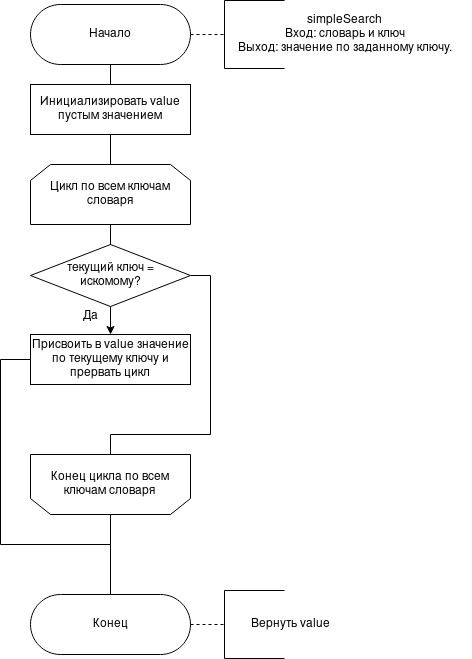
\includegraphics[scale=0.62]{simple_search.jpg}
		\caption{Схема алгоритма полного перебора.}
		\label{fig:mpr}
	\end{figure}
	
	\begin{figure}[H]
		\centering
	%	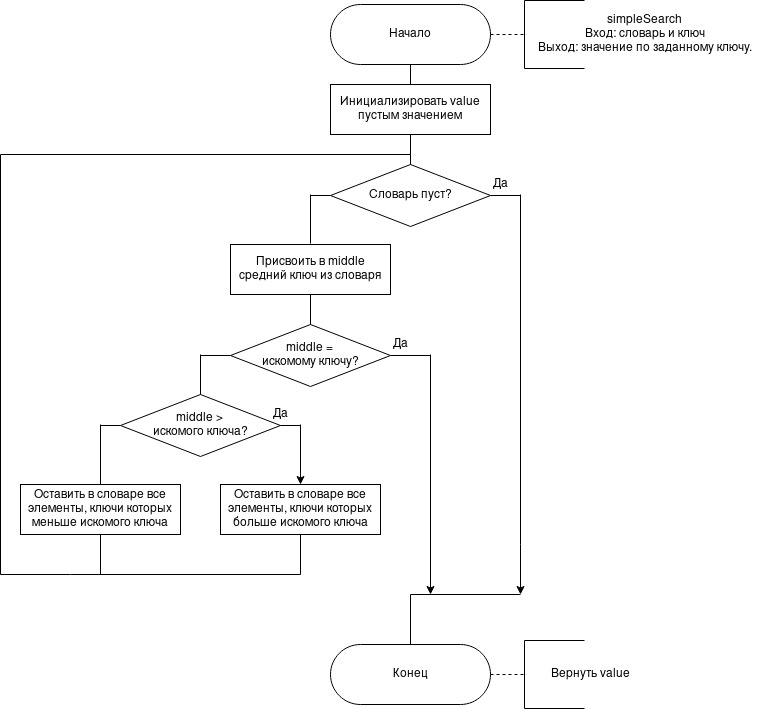
\includegraphics[scale=0.7]{binary_search.jpg}
		\caption{Схема алгоритма двоичного поиска.}
		\label{fig:mpr}
	\end{figure}
	
	\begin{figure}[H]
		\centering
%		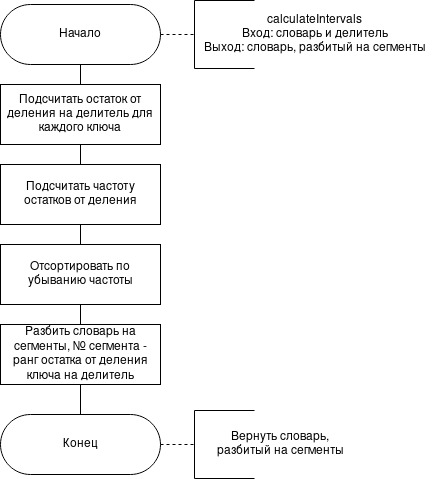
\includegraphics[scale=1]{calculate_intervals.jpg}
		\caption{Схема алгоритма частотного анализа.}
		\label{fig:mpr}
	\end{figure}

	\begin{figure}[H]
		\centering
	%	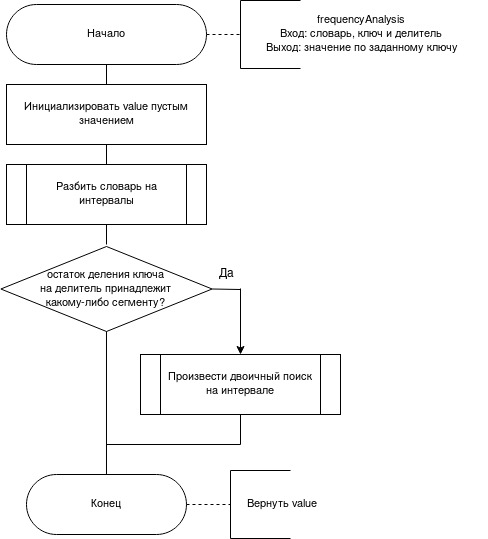
\includegraphics[scale=1]{freq_analysis.jpg}
		\caption{Схема алгоритма поиска с использованием частотного анализа.}
		\label{fig:mpr}
	\end{figure}
	
\section{Автоматическая параметризация}
	
	\section*{Вывод}
	
	На основе теоретических данных, полученных аз аналитического раздела, были построенны схемы алгоритмов для решения задачи коммивояжёра.
	
	\chapter{Технологическая часть}
	
	В данном разделе приведены средства реализации и листинги кода.
	
	\section{Требование к ПО}
	
	К программе предъявляется ряд требований:
	
	\begin{itemize}
		\item на вход подается матрица смежности, со значениями не более чем максимальное целое число деленное пополам;
		\item на выходе -- кратчайший путь.
	\end{itemize}
	
\section{Средства реализации}
	
Для реализации ПО я выбрал язык программирования C++ \cite{C++}. Данный выбор обусловлен моим желанием расширить свои знания в области применения данного языка программирования.
	
\section{Реализация алгоритмов}

В листингах 3.1 - 3.3 представлены листинги алгоритмов решения задачи коммивояжёра.
	
\begin{lstlisting}[label=some-code,caption=123, language=C++]

\end{lstlisting}
	
\begin{lstlisting}[label=some-code,caption=123, language=C++]

\end{lstlisting}

	
\section{Тестовые данные}

В таблице 3.1 приведены тестовые данные. Все тесты были пройденны успешно.

тут таблица
	
\section*{Вывод}
	
В данном разделе была разработаны и протестированны алгоритмы решения задачи коммивояжёра.
	
\chapter{Исследовательская часть}
	
В данном разделе приведен анализ характеристик разработанного ПО.

\section{Технические характеристики}
	
Ниже приведены технические характеристики устройства, на котором было проведено тестирование ПО:
	
\begin{itemize}
	\item Операционная система: Debian \cite{debian} Linux \cite{linux} 11 <<bullseye>> 64-bit.
	\item Оперативная память: 12 GB.
	\item Процессор: Intel(R) Core(TM) i5-3550 CPU @ 3.30GHz \cite{i5}.	
\end{itemize}
	
\section{Время выполнения алгоритмов}
	
Время выполнения алгоритма замерялось с помощью встроенной в С++ стандартной библиотеки std::chrono \cite{std::chrono}.

В таблице 4.1 приведено сравнение времени выполнения алгоритмов.

	
\section*{Вывод}
	

\chapter*{Заключение}
\addcontentsline{toc}{chapter}{Заключение}
	
В рамках данной лабораторной работы лабораторной работы была достигнута её цель: изучен муравьиный алгоритм и приобретены навыки параметризации методов на примере муравьиного алгоритма. Также выполнены следующие задачи:
	
\begin{itemize}
	\item реализованны два алгоритма решения задачи коммивояжера;
	\item замерено время выполнения алгоритмов;
	\item муравьиный алгоритм протестирован на разных переменных;
	\item сделаны выводы на основе проделанной работы;
\end{itemize}

Вывод ???

\addcontentsline{toc}{chapter}{Литература}
\bibliographystyle{utf8gost705u}  % стилевой файл для оформления по ГОСТу
\bibliography{51-biblio}          % имя библиографической базы (bib-файла)
	
\end{document}
